\section*{Задача 976}
Исследовать особые точки. Дать чертеж расположения интегральных кривых на плоскости (x, y).
$$
    \begin{cases}
        x' = 3x + y \\
        y' = y - x
    \end{cases}
$$
\begin{solution}
    $$ |A - \lambda E| = \begin{vmatrix}
            3 - \lambda & 1           \\
            -1            & 1 - \lambda
        \end{vmatrix} = (3-\lambda)(1 - \lambda) + 1 = 3 - 3\lambda - 1\lambda + \lambda^2 + 1 = \lambda^2 - 4\lambda + 4 = (\lambda - 2)^2 = 0
    $$
    $$ \lambda_1 = \lambda_2 = 2 $$
    \begin{figure}[h]

        \centering
        
        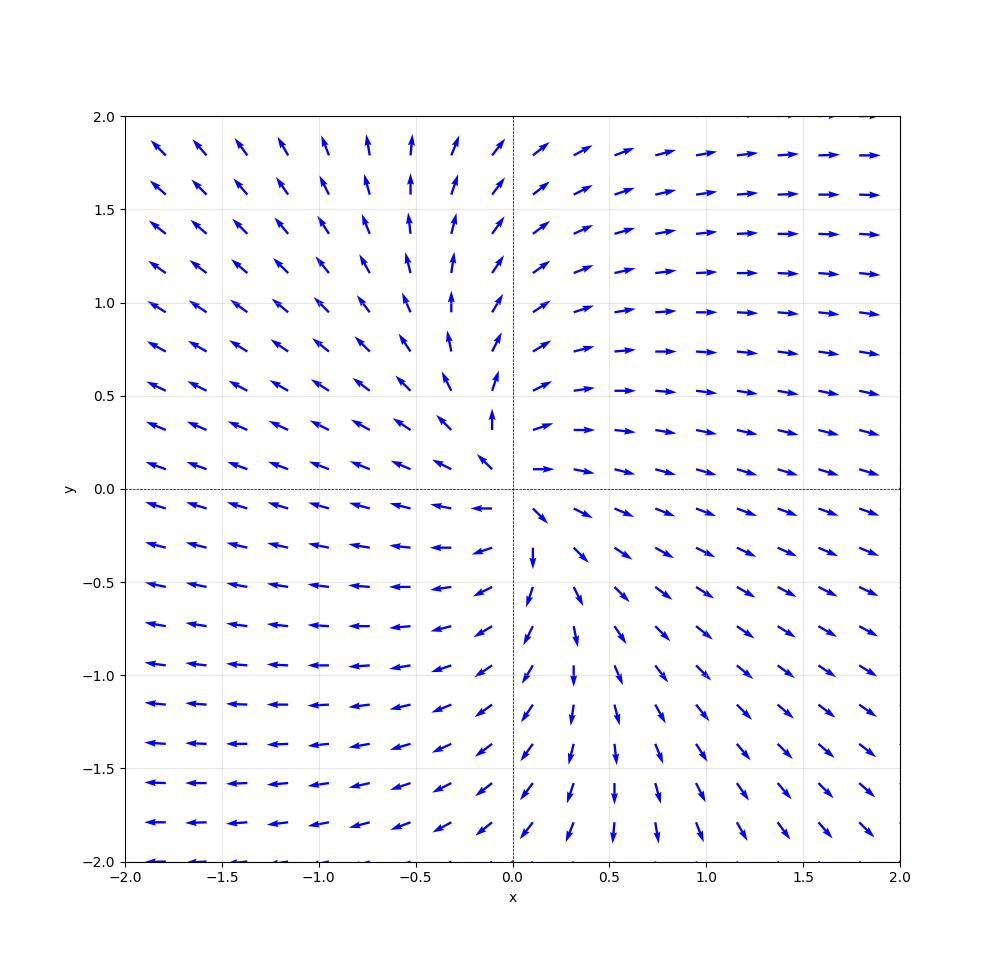
\includegraphics[width=0.8\linewidth]{graph/976.png}
                
        \label{fig:mpr}
        
    \end{figure}

\end{solution}\pagebreak
